\documentclass[11pt,a4paper]{article}
\usepackage{fontspec,xeCJK}
\setCJKmainfont{Noto Serif CJK SC}
\setCJKsansfont{Noto Sans CJK SC}
\usepackage[margin=2.2cm]{geometry}
\usepackage{amsmath,amssymb,booktabs,array,enumitem,xcolor,longtable,float,graphicx,multirow}
\usepackage[hidelinks]{hyperref}
\usepackage{caption}
\captionsetup{font=small,labelsep=quad}
\linespread{1.25}
\setlength{\emergencystretch}{3em}
\setlist{nosep,leftmargin=2em}
\renewcommand{\contentsname}{目录}
\renewcommand{\tablename}{表}
\renewcommand{\figurename}{图}
\newcolumntype{L}[1]{>{\raggedright\arraybackslash}p{#1}}
\newcommand{\ok}{\textcolor{green!45!black}{成立}}
\newcommand{\nok}{\textcolor{red!70!black}{不成立}}
\newcommand{\half}{\textcolor{orange!80!black}{部分成立}}

\title{\textbf{supplement-v13 实验报告与阶段评估}\\[4pt]
\large 完整学习曲线上的三种 oracle：测试复用与结果运气\\[2pt]
\normalsize 本次情况 · 比上次好在哪里 · 目前支持的结论 · 研究主线与偏移 · 论文层次}
\author{整理：Claude}
\date{2026 年 11 月 11 日}

\begin{document}
\maketitle

\section*{一页结论}
\begin{enumerate}
\item \textbf{本次做了什么。}为回应文献核查中发现的 Zhou 等（AISTATS 2021）——他们用独立验证集给 oracle 选样，从而避开测试复用——我们在\textbf{完整学习曲线}上比较了三种 oracle：在测试集上选样的“基准式”（CDALBench、BoSS 的做法）、在独立验证集上选样的“Zhou 式”、以及选样时看不到候选标签的“事前式”。8 个数据集 $\times$ 32 条轨迹，每条 30 步，另有 4 个数据集用 4 倍大的验证集各 16 条。协议运行前冻结，全部完成。
\item \textbf{结果。}4 条登记预测中 2 条成立、2 条不成立。成立的一条是全项目最关键的：所有策略都明显落后于基准式 oracle 的数据集为 8/8，落后于 Zhou 式为 6/8，落后于事前式只有 1/8。\emph{拆分评价集只去掉了测试复用，结论基本不变；把运气也去掉，结论在 7 个数据集上被推翻。}不成立的是：在整条曲线上，运气只在 3/8 个数据集达到实质水平，也不再随标签噪声变化——它集中在学习曲线最前面，标签多了以后就消失。
\item \textbf{比上次好在哪里。}上一轮（v12）的“基准结论被推翻”主要靠描述性证据，登记的主预测只成立一半；这一轮在\textbf{完整学习曲线}上、用\textbf{登记的预测}拿到了同样方向的结论，并且直接回应了“Zhou 已经拆分过评价集”的质疑。
\item \textbf{主线是否偏移。}项目整体经历过一次大的偏移（10 月底的算法论文 $\to$ 11 月 5 日起的评价方法学论文），此后主线稳定：\emph{oracle 差距中有多少是真正能争取的提升空间}。这一轮没有改变主线，但改变了重心：从“偶然性下限随噪声变化”转向“测试复用与运气共同决定基准结论；运气是学习曲线早期现象”。
\item \textbf{论文层次。}目前是一篇方法严谨、实证扎实、概念新颖性一般的评价方法学论文，大致处于 \textbf{CCF-B 会议的录用边缘}（DASFAA 把握约 30--35\%），CCF-C 会议或相关 workshop 把握较大；要进入顶会（如 NeurIPS Datasets \& Benchmarks、ICLR），还缺深度模型和标准基准上的完整复现。
\end{enumerate}

\tableofcontents
\newpage

% ======================================================================
\section{本次实验做了什么}
\subsection{动机}
上一份阶段评估中的文献核查发现：Zhou 等（AISTATS 2021）的模拟退火 oracle 在独立验证集 $D_V$ 上选样、在测试集 $D_T$ 上报告，已经避开了测试复用；而 CDALBench（2024）和 BoSS（2026）原文明确在测试集上选样。审稿人很可能据此质疑：“测试复用早就有人解决了”。另外，v12 的 E2 只在四个历史规模上各做单步，而基准报告的是整条学习曲线。本轮实验同时回答这两个问题：\emph{在完整学习曲线上，拆分评价集之后，还剩多少差距是运气？}

\subsection{设计}
\begin{table}[H]
\centering\small
\begin{tabular}{L{3.2cm}L{11.6cm}}
\toprule
项目 & 设定 \\
\midrule
学习曲线 & 从 68 条已标注数据出发，每步从 40 个新候选中取 10 个，共 30 步，到 368 条；无风险约束、无延迟（池式基准设定） \\
三种 oracle & \textbf{基准式}：用候选的真实标签，在测试集上贪心选样；\textbf{Zhou 式}：同样用真实标签，但在与测试集等大的独立验证集上选样；\textbf{事前式}：在验证集上，按结果模型 $\hat p$ 生成的 32 个标签复本的平均损失选样，选样时看不到候选的真实标签 \\
策略 & Random、Uncertainty、BAIT-greedy、TargetVar-greedy、Fisher-cost（DC-PRISM 可能少取标签，会破坏统一横轴，故未纳入） \\
评分 & 所有曲线都在同一测试集上用真实标签评分；每条曲线沿自己的轨迹累积标签 \\
分解（整条曲线平均 Brier）& 测试复用 = Zhou 式 $-$ 基准式；运气 = 事前式 $-$ Zhou 式；剩余 = 最佳策略 $-$ 事前式 \\
规模 & MAIN：8 数据集 $\times$ 32 条轨迹；BIGV：4 个大数据集，验证集为测试集的 4 倍，各 16 条 \\
学习器 & $\ell_2$ 逻辑回归（与主研究一致） \\
统计 & 配对 $t$、Bonferroni 联合区间与 Holm 校正；实质阈值 $0.5\times10^{-3}$ Brier \\
\bottomrule
\end{tabular}
\end{table}

\subsection{执行情况}
\begin{itemize}
\item \textbf{流程}：协议与 7 个源文件的哈希在运行前冻结（本地提交 \texttt{97be653}），冒烟测试只用开发种子 99001，测时只用 99003；正式种子 171001--172016 均为首次使用。
\item \textbf{运行}：MAIN 256 条轨迹用时 85 分钟，BIGV 64 条用时 20 分钟，全部 COMPLETE；结果提交为 \texttt{e6ead75}。
\item \textbf{文件}：代码 \nolinkurl{experiments/supplement_v13/}，协议 \nolinkurl{configs/supplement_v13.json}，结果与预测核对 \texttt{results/supplement\_v13/\{MAIN,BIGV\}/}。
\end{itemize}

% ======================================================================
\section{结果}
\subsection{登记预测核对}
\begin{table}[H]
\centering\small
\begin{tabular}{L{1.0cm}L{8.2cm}L{1.8cm}L{3.6cm}}
\toprule
编号 & 预测 & 结果 & 实际 \\
\midrule
P1 & 拆分评价集后，运气在噪声最高的 4 个数据集上都达到实质水平；运气占比与噪声正相关 & \nok & 4 个中 2 个（LC、PPDai）；全部 8 个中 3 个；Spearman 0.19 \\
P2 & 测试复用占比在曲线后段（第 21--30 步）大于前段（第 1--10 步），至少 6/8 & \ok & 8/8 \\
P3 & 所有策略都明显落后于基准式 oracle：8/8；落后于 Zhou 式：$\ge6/8$；落后于事前式：$\le4/8$ & \ok & 8/8、6/8、1/8 \\
P4 & 验证集放大 4 倍后，运气在至少 3/4 个数据集上达到实质水平 & \nok & 2/4（LC、UCI），4/4 为正 \\
\bottomrule
\end{tabular}
\end{table}

\subsection{各数据集的分解}
\begin{table}[H]
\centering\small
\footnotesize\caption{整条学习曲线上，基准式 oracle 对最佳策略的领先及其构成（逻辑回归，32 条轨迹/数据集；$\times10^{-3}$ Brier）。最后一列：所有策略是否都明显落后于 基准式/Zhou 式/事前式 oracle。}
\setlength{\tabcolsep}{3pt}
\begin{tabular}{lrrrrrlll}
\toprule
数据集 & 噪声 & 领先 & 复用\% & 运气\% & 剩余\% & 运气检验 & 复用\% 前段$\to$后段 & 都落后？ \\
\midrule
Spambase & 0.052 & 7.9 & 58 & 23 & 18 & 实质 & 41$\to$75 & 是/是/否 \\
USPS & 0.067 & 14.0 & 38 & 3 & 59 & 不确定 & 23$\to$54 & 是/是/是 \\
再入院 & 0.080 & 2.9 & 56 & 27 & 17 & 正，未达阈值 & 35$\to$81 & 是/是/否 \\
银行营销 & 0.091 & 4.6 & 54 & 17 & 29 & 正，未达阈值 & 32$\to$92 & 是/否/否 \\
HMEQ & 0.097 & 4.9 & 66 & 3 & 31 & 不确定 & 38$\to$103 & 是/否/否 \\
PPDai & 0.106 & 4.5 & 35 & 32 & 33 & 实质 & 23$\to$50 & 是/是/否 \\
UCI Credit & 0.136 & 7.0 & 45 & 19 & 36 & 正，未达阈值 & 28$\to$71 & 是/是/否 \\
LendingClub & 0.143 & 5.3 & 50 & 31 & 19 & 实质 & 30$\to$87 & 是/是/否 \\
\bottomrule
\end{tabular}
\end{table}
\noindent 注：后段 HMEQ 的复用占比超过 100\%，是因为后段运气为负值（事前式略好于 Zhou 式），属于抽样波动。“最佳策略”按数据集事后选出，属描述性。

\begin{figure}[H]
\centering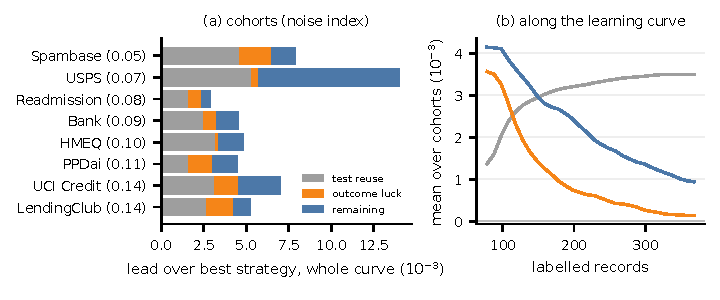
\includegraphics[width=\linewidth]{figures/fig_curves.pdf}
\caption{(a) 各数据集整条曲线上基准式 oracle 领先的构成：测试复用（灰）、运气（橙）、剩余（蓝）。(b) 三部分沿学习曲线的变化（各数据集平均，三步滑动平均）。运气在最初约 3.5$\times10^{-3}$，到 200 条左右基本消失；测试复用一路上升。}
\end{figure}

\subsection{要点}
\begin{enumerate}
\item \textbf{结论被改变，而且是登记的。}对照基准式 oracle，40/40 个“数据集--策略”对都明显落后；对照 Zhou 式，36/40；对照事前式，17/40（8 个数据集中只有 USPS 仍然全部落后）。
\item \textbf{测试复用是整条曲线上最大的一块}（35--66\%），而且越往后越大（8/8）。验证集放大 4 倍后，复用缩小 28--52\%，说明它主要来自在有限评价集上选样的噪声。
\item \textbf{运气是学习曲线早期的现象。}前 10 步里，运气占 Zhou 式 oracle 领先的 31--71\%（信贷、再入院与营销数据集）；后期基本为零。所以整条曲线平均下来，它只在 3/8 个数据集达到实质水平，而且不再随噪声变化。
\item \textbf{近确定标签上，oracle 的领先大多是真的。}USPS 上剩余部分占 59\%，所有策略对三种 oracle 都明显落后——与单步研究一致。
\end{enumerate}

% ======================================================================
\section{比上次好在哪里}
\subsection{与 v12（11 月 10 日）对比}
\begin{longtable}{L{3.0cm}L{5.2cm}L{5.2cm}L{1.3cm}}
\toprule
问题 & v12 的状况 & v13 之后 & 变化 \\
\midrule\endhead
“基准结论被改变”的证据 & 主要是描述性的（逐点区间）；登记主预测只成立一半 & 完整学习曲线上，登记预测 P3 成立（8/8$\to$6/8$\to$1/8） & \textbf{变强} \\
与 Zhou 2021 的关系 & 没有比较，审稿人会说“复用早已解决” & 直接比较：拆分评价集后结论在 6/8 个数据集上仍成立，必须同时去掉运气 & \textbf{新增} \\
单步 vs 完整曲线 & 只有四个位置的单步 & 30 步完整轨迹，每种方法沿自己的轨迹累积标签 & \textbf{新增} \\
测试复用随曲线变化 & 单步中描述性观察 & 登记预测成立（8/8） & 变强 \\
验证集大小 & 未检验 & 4 倍验证集：复用缩小，运气仍为正 & 新增 \\
运气随噪声的规律 & 单步中稳健（Spearman 0.81--0.88） & 整条曲线上不成立（0.19）；运气集中在早期 & \textbf{变弱} \\
\end{longtable}

\subsection{与项目早期相比}
\begin{table}[H]
\centering\small
\begin{tabular}{L{2.6cm}L{6.0cm}L{6.4cm}}
\toprule
阶段 & 主要主张 & 证据状况 \\
\midrule
10 月底--11/03 & DC-PRISM 优于基线 & 真实数据新种子确认 1/12 显著；放弃 \\
11/05--11/06 & oracle 差距存在偶然性下限 & 估计量混用、只验证到 12 候选、没有基准层面的证据 \\
11/10（v12） & 残差稳健；后期基准结论可能是假象 & 四个漏洞补齐；基准证据为描述性 \\
\textbf{11/11（v13）} & 拆分评价集不够，去掉运气后基准结论改变 & 完整学习曲线上的登记证据；回应已有工作 \\
\bottomrule
\end{tabular}
\end{table}

% ======================================================================
\section{目前支持什么结论}
\subsection{有强证据支持（多轮独立研究、登记预测、稳健性检验）}
\begin{enumerate}
\item \textbf{oracle 报告的领先不能直接当作提升空间。}在 8 个数据集、单步与完整学习曲线、风险约束与无约束设定下，都有相当部分是任何策略拿不到的（测试复用 + 运气）。
\item \textbf{只拆分评价集不够。}按 Zhou 的做法拆分后，“所有策略都明显落后”在 6/8 个数据集仍成立；去掉运气后只剩 1/8（v13，登记）。
\item \textbf{在单步（以及学习曲线早期），运气占比随标签噪声上升。}跨数据集（两批新状态，Spearman 0.81--0.88）、数据集内注入噪声（3/3）、五种结果模型下都成立；近确定标签 10--16\%，噪声大的信贷 50--60\%。
\item \textbf{这些结论不是方法缺陷造成的。}穷举到 20 候选与贪心差 $\le0.11\times10^{-3}$；更强的事前搜索只多拿 0.5\%；残差区间两端很窄。
\item \textbf{测试复用随学习曲线增大。}单步研究和完整曲线（登记，8/8）都显示后期报告差距的大部分是复用。
\end{enumerate}

\subsection{有证据但有条件}
\begin{enumerate}
\item \textbf{近确定标签上 oracle 的领先大多是真的}（USPS：剩余 59\%，对三种 oracle 都落后）——只在一个手写数字数据集上检验。
\item \textbf{信息代理只在匹配学习器时有用}——风险约束案例研究中的结论。
\end{enumerate}

\subsection{不支持或已撤回}
\begin{enumerate}
\item \textbf{在整条学习曲线上运气随噪声变化}：不支持（v13 P1 不成立，Spearman 0.19）。
\item \textbf{运气在整条曲线上普遍达到实质水平}：不支持（3/8；放大验证集后 2/4）。
\item \textbf{DC-PRISM 普遍优于强基线}：不支持。
\item 早期说法“下限占比 79\%”“独立正态上界”“领先 4.48$\to$1.25”：已撤回。
\end{enumerate}

% ======================================================================
\section{研究主线与偏移}
\subsection{当前主线（一句话）}
\emph{主动学习基准用 oracle 衡量提升空间，但 oracle 的领先中有两块是任何策略都拿不到的——在有限评价集上选样造成的测试复用，以及所获标签中的结果运气；前者随学习曲线增大，后者集中在曲线早期并随标签噪声增大；两块一起去掉之后，“实用策略明显落后于 oracle”这一基准结论在多数数据集上不再成立。}

\subsection{是否偏移}
\begin{longtable}{L{2.4cm}L{6.0cm}L{6.6cm}}
\toprule
时间 & 主线 & 偏移性质 \\
\midrule\endhead
10 月底 & 风险约束、延迟反馈下的标签获取算法 DC-PRISM & 起点 \\
11/04--05 & 收益机制：事后提升空间多少可事前获得 & \textbf{大偏移}：从算法转向机制，原因是算法在真实数据上没有稳定优势 \\
11/05--06 & oracle 差距存在偶然性下限 & 中等偏移：从“我们的场景”推广到“主动学习评价” \\
11/10 & oracle 差距中有多少是提升空间：复用 + 运气 & 小调整：估计量统一，加入测试复用 \\
11/11 & 同上；运气是早期现象，拆分评价集不够 & \textbf{没有偏移}，重心调整：从“下限随噪声变化”转向“两块一起决定基准结论” \\
\end{longtable}

\paragraph{判断。}项目在 11 月 5 日前后发生过一次实质性偏移（算法 $\to$ 评价方法学），这是被证据推动的、合理的偏移；之后的一周主线稳定，每一轮实验都在加固同一个问题。需要注意两点：
\begin{itemize}
\item \textbf{应用场景与主线的张力}：风险约束、延迟反馈和 DC-PRISM 来自最初的信贷场景，现在只是案例研究；论文中这部分越来越像附录。如果继续加强基准方向，可以考虑进一步弱化或移出 DC-PRISM。
\item \textbf{“运气”的地位下降}：v13 显示在整条曲线上测试复用比运气更大、更稳定。论文题目和摘要如果继续把“结果运气”放在核心位置，需要明确它主要是早期和单步现象。
\end{itemize}

% ======================================================================
\section{论文大概是什么层次}
\subsection{评估}
\begin{table}[H]
\centering\small
\begin{tabular}{L{3.8cm}cL{9.4cm}}
\toprule
维度 & 水平 & 说明 \\
\midrule
实验规范与严谨度 & 高 & 冻结协议、登记预测、多重比较、穷举核验、负结果如实报告，明显高于同类会议论文 \\
实证发现 & 中偏高 & “拆分评价集不够、去掉运气后基准结论改变”是新的、对当前基准（CDALBench、BoSS）有直接含义的发现 \\
概念与理论 & 低 & 完全信息价值、乐观偏差、测试集过拟合都已有人讲过；上下界证明简单 \\
外部有效性 & 中偏低 & 表格数据、逻辑回归/单隐层网络、小候选池；没有深度视觉/文本模型和标准基准的完整复现 \\
写作与一致性 & 中偏高 & 估计量已统一；但题目与摘要的重心需要随 v13 调整 \\
\bottomrule
\end{tabular}
\end{table}

\subsection{对应的发表层次}
\begin{table}[H]
\centering\small
\begin{tabular}{L{5.2cm}cL{7.2cm}}
\toprule
目标 & 把握（主观） & 理由 \\
\midrule
CCF-C 会议 / 相关 workshop & 较高（60\% 以上） & 严谨度和发现都足够 \\
DASFAA 等 CCF-B 会议 & 约 30--35\% & 录用边缘：严谨但概念新颖性一般；受众对主动学习评价不一定熟悉 \\
数据挖掘/机器学习期刊（如 DMKD、TMLR 类） & 中等 & 期刊更看重严谨与完整性，篇幅也允许写全；需要补深度模型 \\
顶会（NeurIPS D\&B、ICLR 等） & 较低（$<$15\%） & 缺深度模型、标准基准完整复现和更强的理论 \\
\bottomrule
\end{tabular}
\end{table}

\paragraph{总体判断。}这是一篇 \textbf{CCF-B 会议边缘、CCF-C 稳妥} 的评价方法学论文。从 11 月 10 日上午的约 15--20\% 到现在的约 30--35\%，提升来自两点：方法学漏洞全部补齐、拿到了登记的“基准结论被改变”证据。要再上一个层次，最有效的一步是在深度模型和一个标准基准（例如 CDALBench 的一个视觉任务）上复现“拆分评价集不够”的结论；但这需要 GPU 时间，在 11 月 25 日截稿前做完的可能性不大。

% ======================================================================
\section{当前状态与待办}
\begin{itemize}
\item \textbf{GitHub}：本地领先 5 个提交（v12 冻结、v12 结果、v12 论文、v13 冻结、v13 结果），尚未推送，等你确认。
\item \textbf{论文}：按你的要求暂不改论文。英文修订稿在此之前已补引 Zhou 2021、Koshorek 2019、Capability Frontier，并加入了 v13 一节（16 页），这些改动尚未提交；中文稿只补了引文。如不需要可以撤回。
\item \textbf{报告文件夹}：本报告、上一份阶段评估、v12 结果说明、改进计划、研究报告，以及 v12 的中英文论文 PDF。
\end{itemize}
\end{document}
